\documentclass[a4paper,12pt]{article}

\usepackage{tma}
\usepackage{hyperref}
\usepackage{graphicx,subfigure}
\usepackage{epstopdf} %%package to overcome problem with eps in pdf files

\graphicspath{{./image/}}


\myname{Anshul Mittal}
\mypin{13113017}
\mycourse{CSN-212: Assignment4}
% \mytma{01}

%\marginnotes

\begin{document}
\begin{center}
    \textbf{Code: Convex Hull}--\href{https://github.com/anshumitts/CSN212/tree/master/Ass4}{Click here}\newline
    Link contains: 
    \begin{itemize}
    	\item main code file (converhull.py).
    	\item output for different number of inputs.
        \item Plot of time vs input length (n) (see fig. \ref{fig:6}.)
    \end{itemize}
    \begin{figure}[ht!]
    \centering
        \subfigure[n=100]{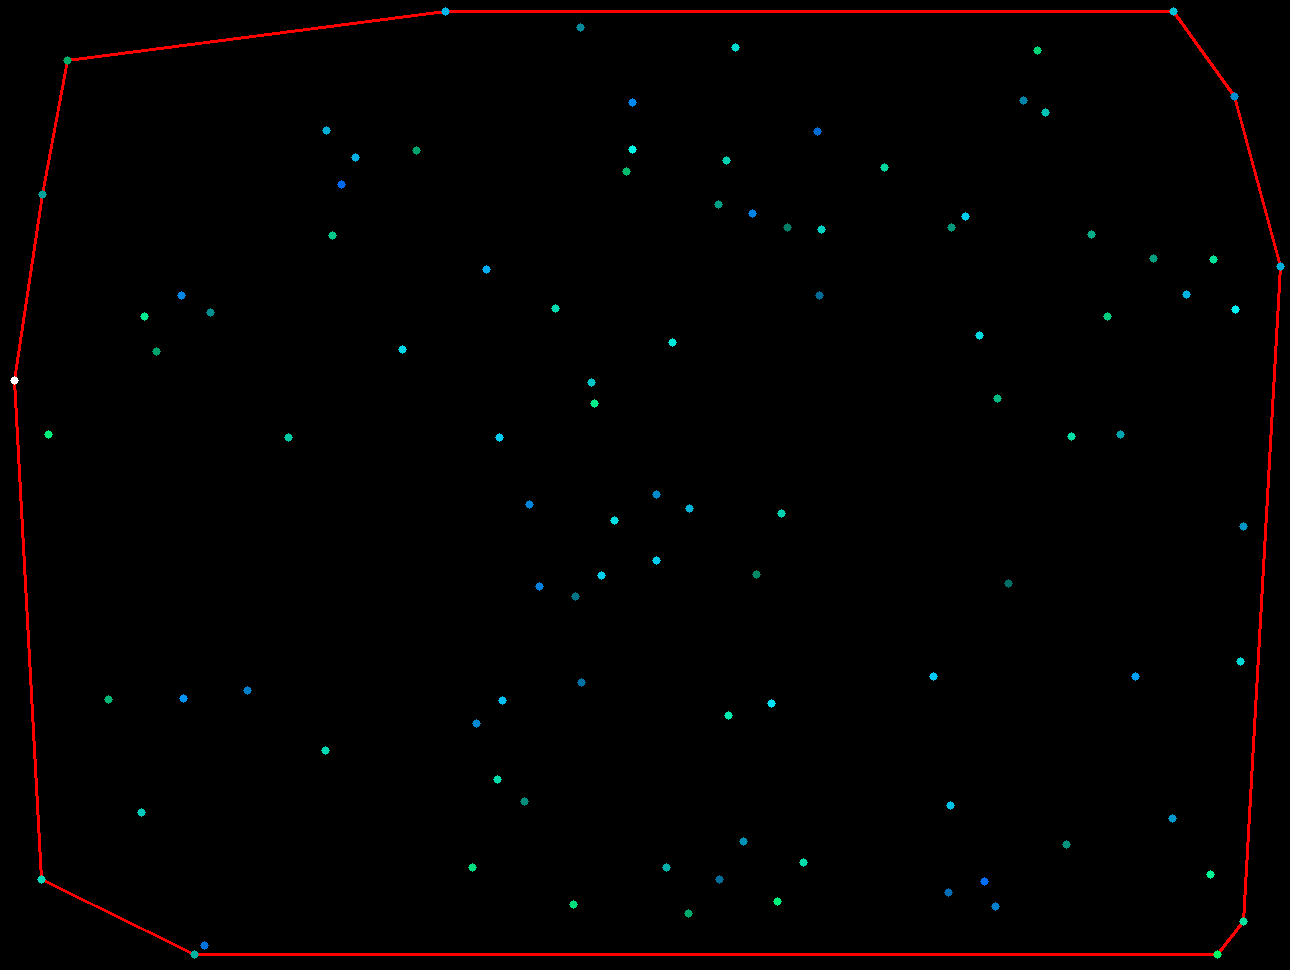
\includegraphics[width=0.4\textwidth]{1}}
        \subfigure[n=1000]{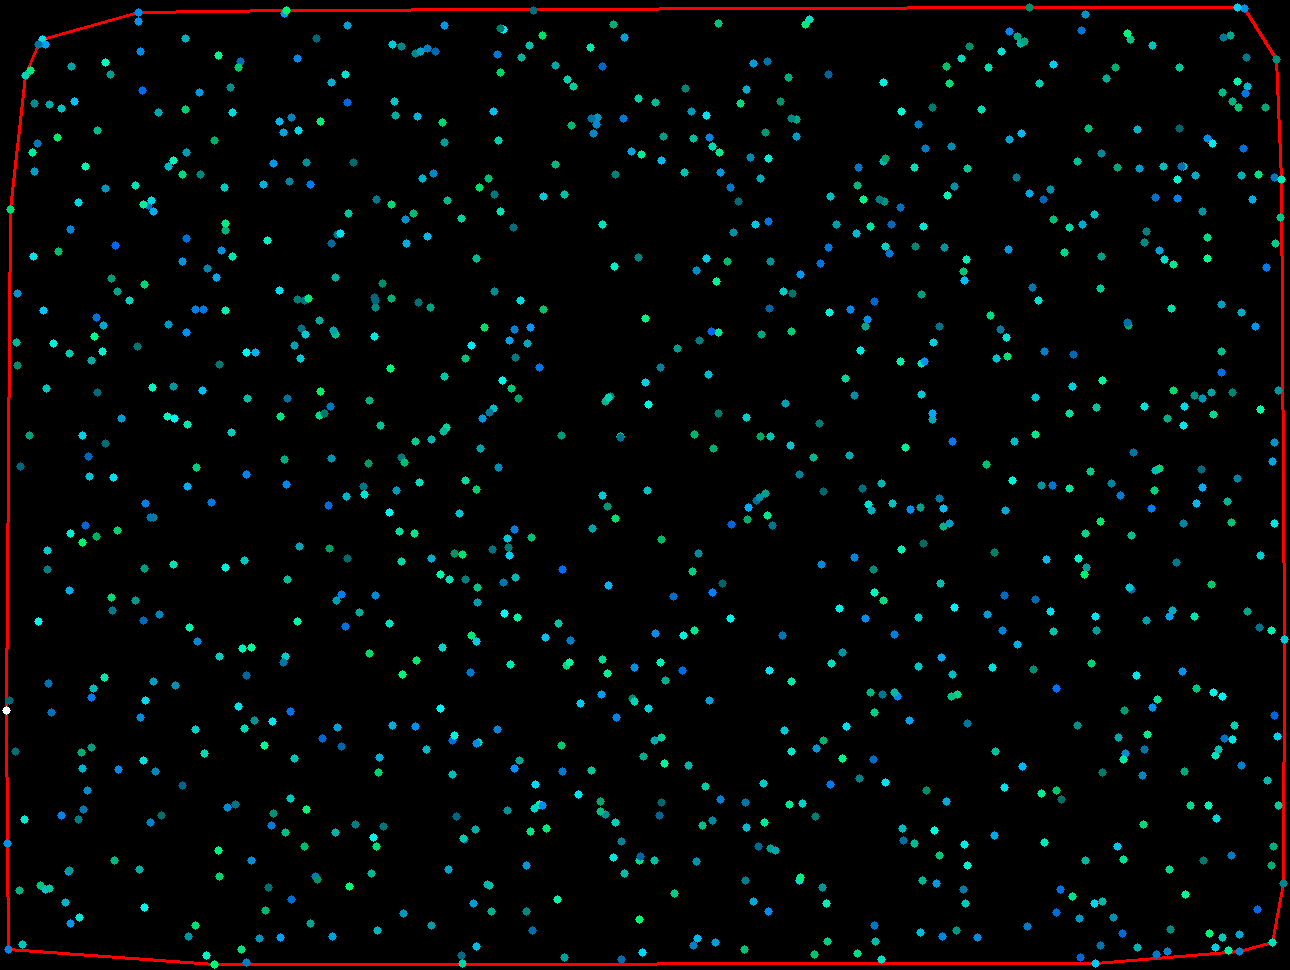
\includegraphics[width=0.4\textwidth]{2}}
        \subfigure[n=2000]{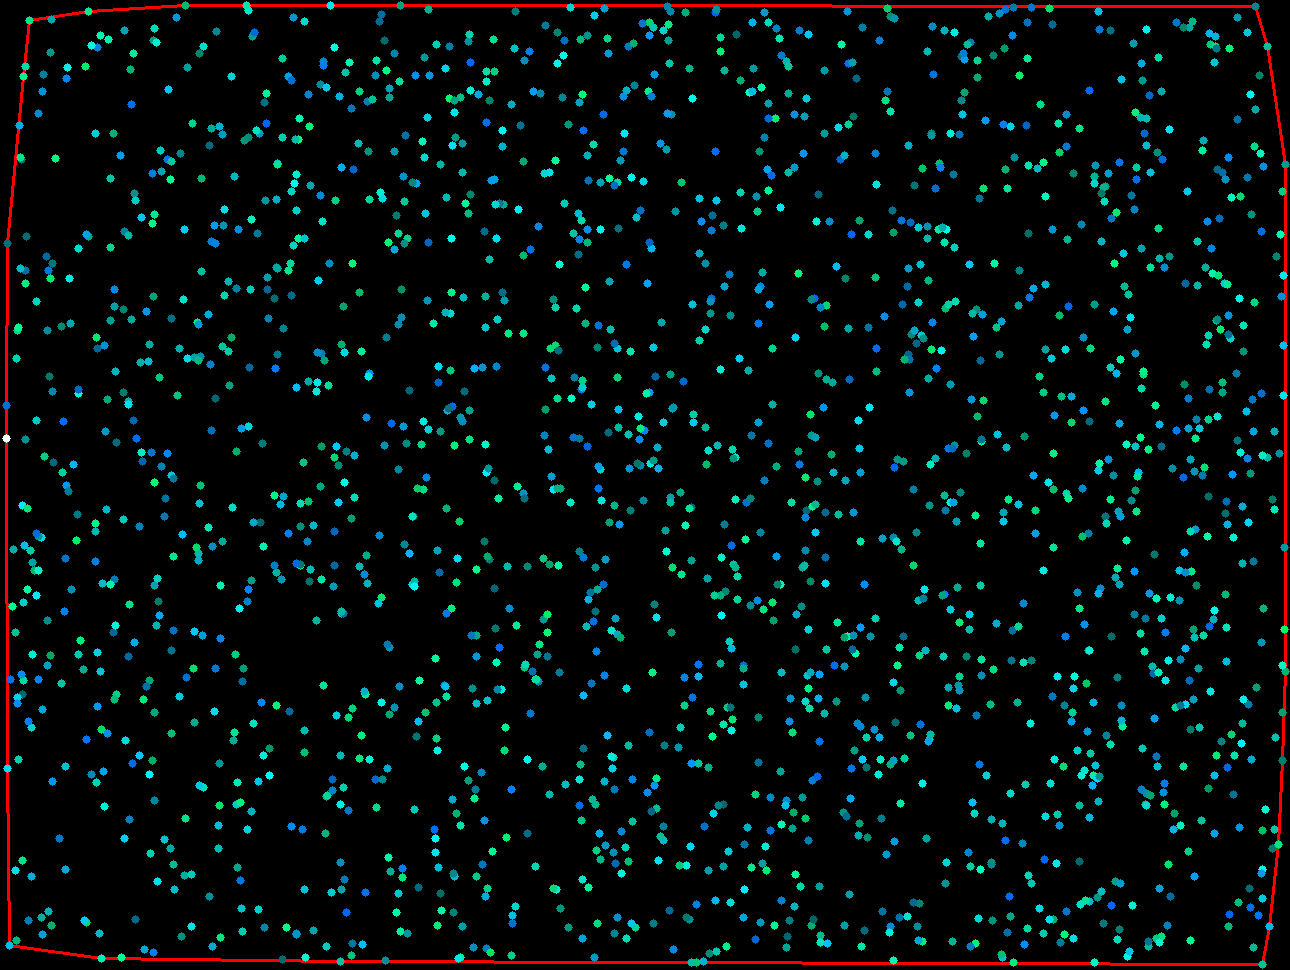
\includegraphics[width=0.4\textwidth]{3}}
        \subfigure[n=5000]{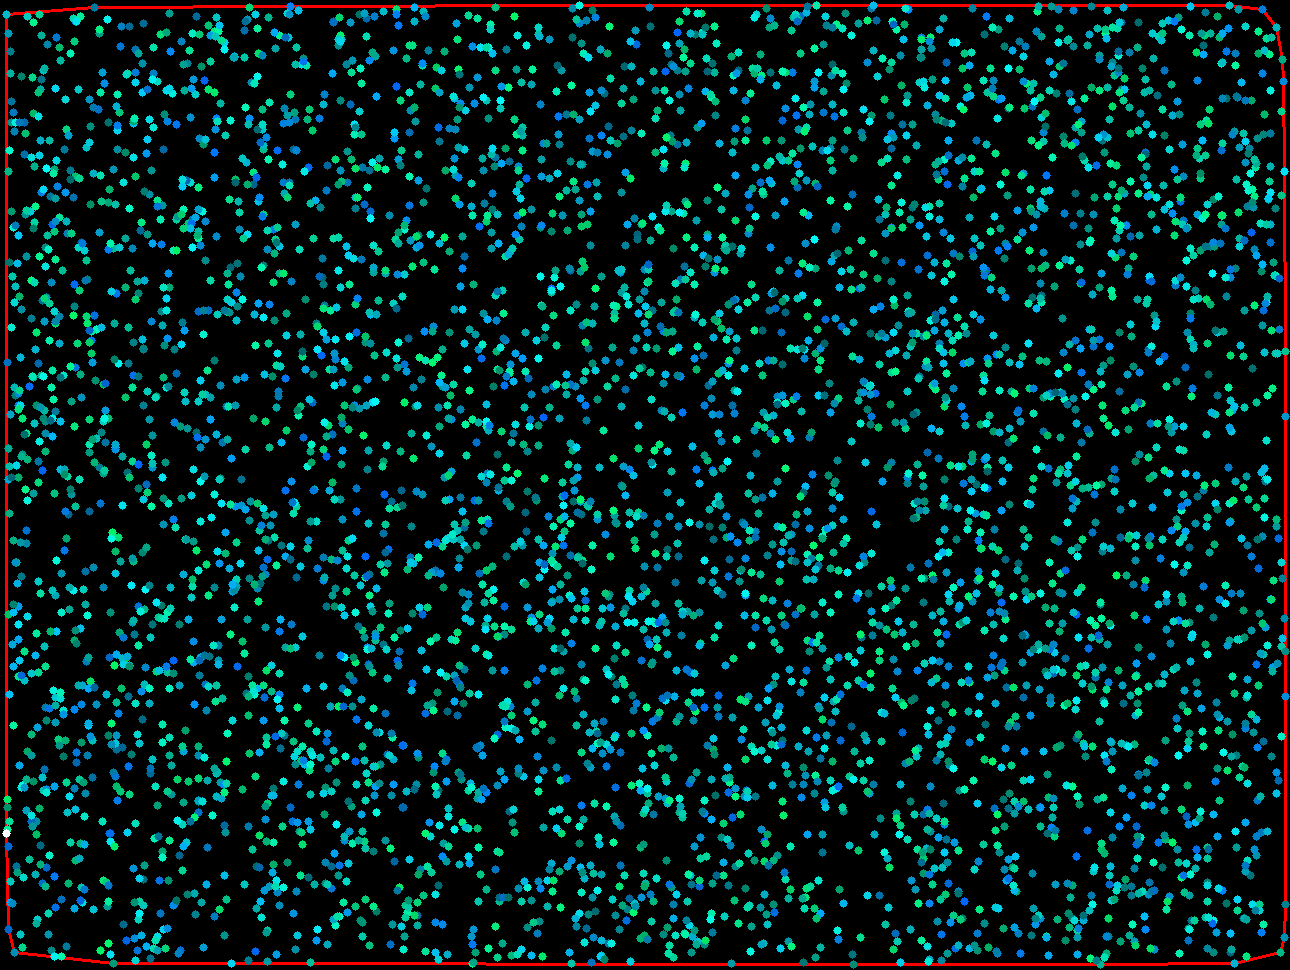
\includegraphics[width=0.4\textwidth]{4}}
        \subfigure[n=10000]{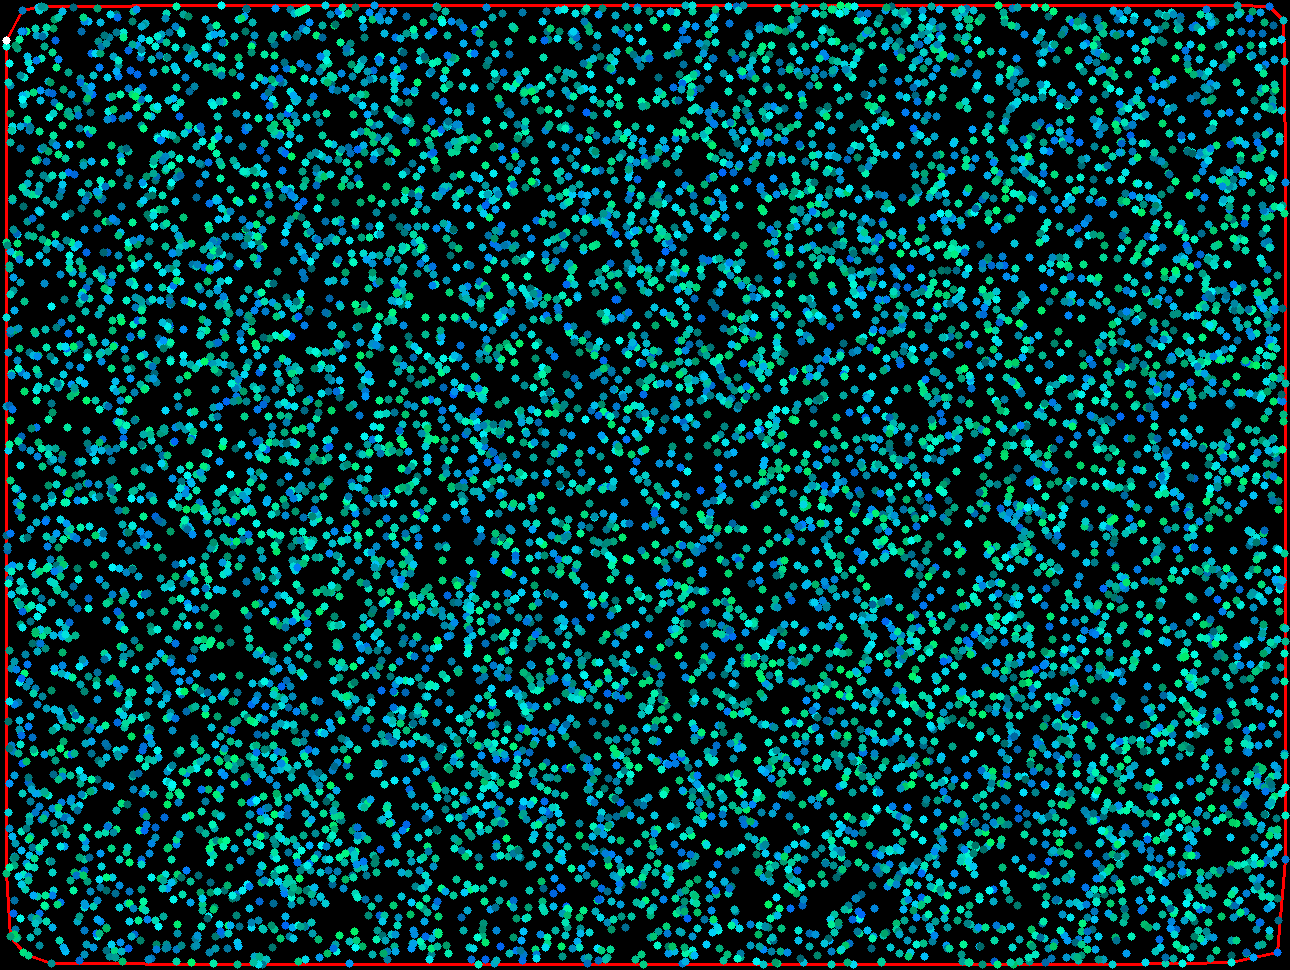
\includegraphics[width=0.4\textwidth]{5}}
    \caption{Output for convex hull for gift wrap, grahm search and quick hull}
    \end{figure}
    \begin{figure}[!h]
        \centering
        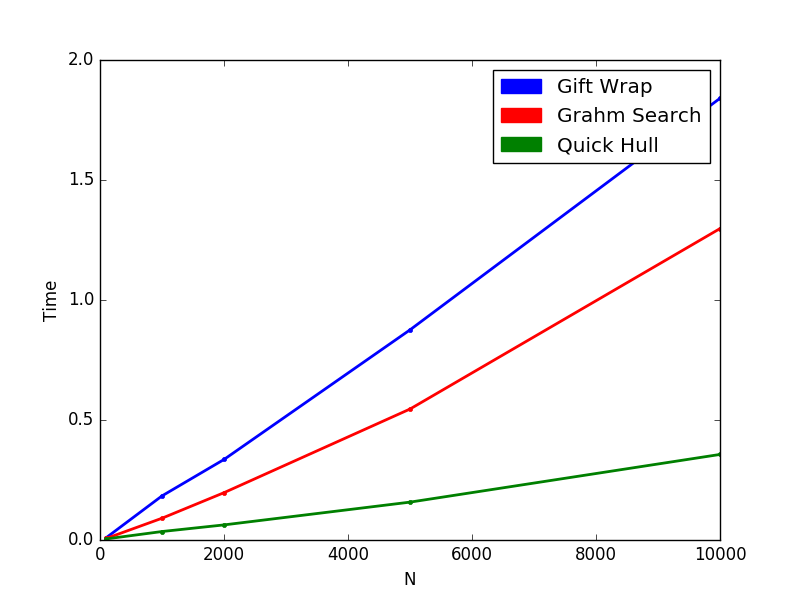
\includegraphics[width=0.72\textwidth]{6}
        \caption{Plot of time(ms) vs number of points(n) for gift wrap, grahm search and quick hull }
        \label{fig:6}
    \end{figure}
\end{center}
\end{document}

